%%%%%%%%%%%%%%%%%%%%%%%%%%%%%%%%%%%%%%
\section{Introduction} \label{intro}
%%%%%%%%%%%%%%%%%%%%%%%%%%%%%%%%%%%%%%
% \todo{
% \begin{enumerate}
%     \item Fix Mitch's headshot photo
%     \item revolute joint constraint definition
%     \item emphasize that we use data to capture the hardest-to-model parts of the system: joint friction and tolerancing/slop/clearance
% \end{enumerate}
% }
\begin{figure}
    %\centering
    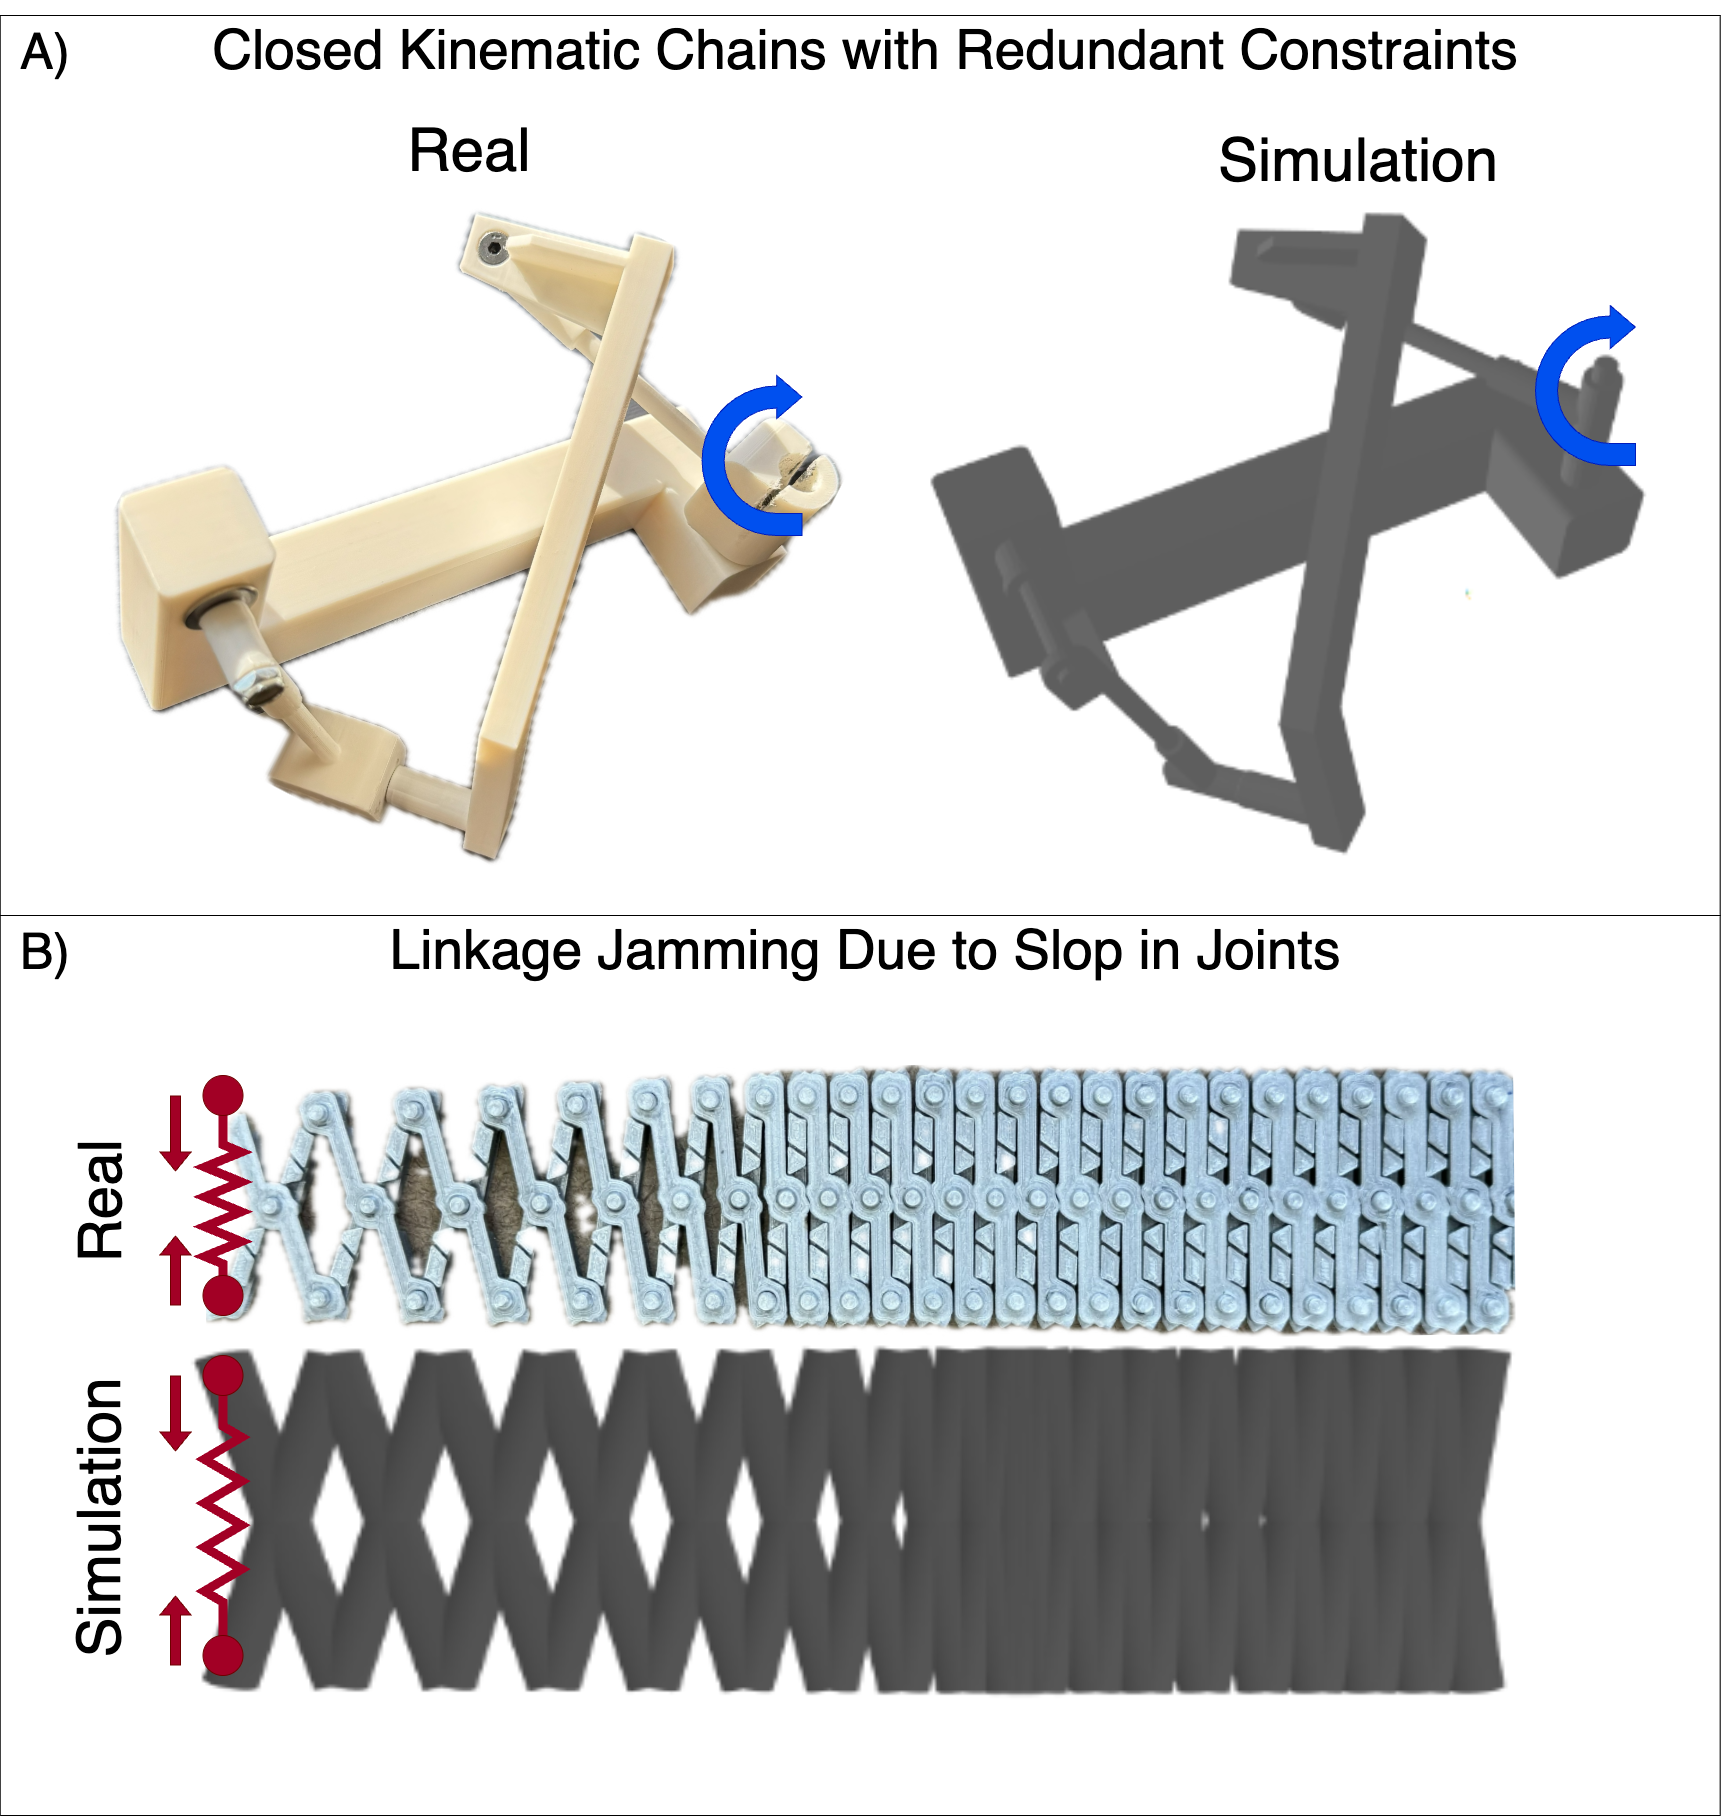
\includegraphics[width=\linewidth]{Figures/scissor_slop.drawio.png}
    \caption{Two examples of complex mechanisms—(A) a Bennett linkage and (B) a jamming scissor mechanism—demonstrating both real and simulated models. These mechanisms' joint clearance and friction can be characterized through a digital twin pipeline, which improves model predictiveness. Our system leverages sensor data from physical prototypes alongside a physics engine, allowing it to learn key parameters such as joint slop and dynamic interaction, enabling accurate simulations and predictive modeling of mechanical behavior.}
    \label{fig:Hero-Figure}
\end{figure}
Linkage mechanisms play a crucial role in the design of deployable space structures, as demonstrated by the intricate mechanisms used in the James Webb Telescope (JWST). The JWST features highly complex deployment mechanisms designed to pack into the Ariane 5 rocket and deploy when released into space. However, these mechanisms introduce significant risks, with some estimates identifying 344 potential single-point failures \cite{menzel_lessons_2024}. Ensuring the success of such a mission necessitates extensive testing, which is time consuming and resource intensive. With systems like the JWST, failure of linkage deployment is one of the aspects tested intensely on Earth before launch. While JWST was successful, Rivera et al. reviewed failures in spacecraft deployable systems in many other instances and cited jamming due to linkage friction or unexpected loads as key examples \cite{rivera_study_2021}. 

Simulation tools offer a valuable resource that allows engineers to analyze system behavior without physical prototypes. Recent advancements in robotics simulation, exemplified by software tools like MuJoCo \cite{todorov_mujoco_2012} and Isaac Sim \cite{mittal_orbit_2023}, have significantly enhanced engineers’ ability to test designs and control algorithms before risking hardware. However, these simulations often fail to fully capture real-world behavior, commonly referred to as the ``sim-to-real gap.''

One solution to the sim-to-real gap is digital twins, which integrate data from the physical world, enabling feedback between the physical system and its virtual counterpart \cite{tao_digital_2019}. Using real-world data with machine-learning algorithms and/or advanced modeling techniques, digital twins provide a more accurate representation of the system in operation \cite{phanden_review_2021}. This synchronization allows engineers to refine simulations, account for unexpected variations, and optimize control or design \cite{ritto_digital_2021, kapteyn_data-driven_2022}. Consequently, digital twins have the potential to play a crucial role in enhancing the fidelity and reliability of linkage-based systems across various development stages.

A key challenge for rigid-body simulators is handling linkages with redundant constraints, joint clearance, and joint friction, which leads to the need for bespoke solutions for complex linkages. Redundant constraints can cause numerical instability, making accurate simulation difficult. Prior work from Wojtyra et al.,  provided analytic conditions for determining uniquely solvable reaction forces in systems with redundant nonholonomic constraints \cite{wojtyra_joint_2009}. Wojtyra et al., later presented a mathematical framework for identifying and calculating joint reactions in mechanisms with dependent constraints due to redundancy or singular configurations \cite{wojtyra_solvability_2013}. To reduce the ill-conditioning, Pekal et al., compared several numerical approaches such as SVD, QR, and nullspace methods \cite{pekal_constraint-matrix-based_2023}. 

In addition, joint friction and joint clearances --- also called ``slop'' or ``tolerance'' --- that arise from manufacturing errors or mechanism wear limit the accuracy of existing simulators. Prior work has explored improving the dynamic modeling of specific linkage configurations with joint clearance \cite{funabashi_dynamic_1978, soong_theoretical_1990} but fail to extend to general linkages.  More recent work has focused on contact force modeling and characterizing the influence on linkage operation \cite{akhadkar_influence_2014, tan_continuous_2017}. In a different approach, some prior work explicitly includes joint clearances into the design process, where they then evaluate linkage trajectory purely kinematically  \cite{mutawe_designing_2012, qi_synthesis_2023}.

% Funabashi et al. systematically analyzed the dynamic behavior of multilink mechanisms with joint clearances, incorporating elastic deformations and friction \cite{noauthor_dynamic_nodate}. Soong et al. developed an analytical model to predict the dynamic behavior of a slider-crank mechanism with radial clearance in its joints \cite{soong_theoretical_1990}. Akhadkar et al. analyzed the impact of joint clearances on the performance of multibody systems by modeling the contact forces in pin and hole assemblies \cite{Akhadkar_influence_2014}. Tan et al. developed a continuous analysis method to investigate dynamic responses in planar mechanisms with clearance, focusing on how joint contact and friction influence the system's motion \cite{tan_continuous_2017}. Mutawe et al. addressed path generation for four-bar linkages under joint clearance constraints and developed a design synthesis method that accounted for joint tolerances, ensuring that mechanisms could achieve specified paths within defined tolerance limits\cite{mutawe_designing_2012}. Qi et al. proposed a method to introduce joint clearances in overconstrained linkages to prevent jamming due to component deformation \cite{qi_synthesis_2023}.  Dupont et al. explored the relationship between Coulomb friction and jamming in rigid-body dynamics \cite{dupont_jamming_1994}. 

While previous work has focused on theoretical outcomes or the characterization of specific linkage configurations~\cite{funabashi_dynamic_1978, soong_theoretical_1990, dupont_jamming_1994, akhadkar_influence_2014, tan_continuous_2017}, this paper introduces a generalizable framework for creating digital twins for linkage analysis. Our approach extends traditional rigid body dynamics simulations by incorporating data-driven parameter estimation from the target mechanism. The proposed framework integrates computer-aided design (CAD), a differentiable simulator, and real-world data to build a data-driven, physics-based digital twin for linkage mechanisms. From the CAD software, the linkage is exported, along with its geometry and physical properties, into a differentiable physics engine that operates using maximal coordinates. Redundant constraints are removed systematically through singular-value decomposition (SVD). Real-world position data is then used to fit joint clearance and damping values for dynamic analysis. These fit parameters are applied in simulations to evaluate system behavior under unseen loads, including detecting jamming. We demonstrate this approach with both simulated and real examples of multi-link scissor mechanisms, as shown in Figure \ref{fig:Hero-Figure}.
% While prior work focused on theoretical results or the characterization of specific linkage configurations, this work presents a generalizable framework for creating digital twins for linkage analysis. Our work extends on a nominal rigid body dynamics simulation through data-driven parameter estimation from target mechanism data. The framework presented in this paper combines computer-aided design (CAD), a differentiable simulator, and real-world data to develop a data-driven physics-based digital twin for the linkage mechanism. A CAD-designed linkage is exported with geometry and physical parameters to a modified differentiable physics engine using maximal coordinates. Redundant constraints are systematically removed via singular value decomposition (SVD). Real-world position data enables optimization of joint clearance and damping for dynamic analysis. These parameters are then applied to simulate the system under unseen loads, evaluating potential jamming scenarios that can be detected through the SVD. We demonstrate our approach using simulated and real examples of multi-link scissor mechanisms seen in Figure \ref{fig:Hero-Figure}.

% Our methodology enables dynamic simulation of linkages with many redundant constraints, providing a robust framework for analyzing and designing complex mechanisms like those found in the JWST. We demonstrate our approach on several interesting linkage examples including several scissor mechanism variants, the Jansen linkage, and a hierarchical linkage mechanism combining a Kresling and scissor system together. 

% Furthermore, our approach allows us to investigate the impact of manufacturing tolerances on linkage performance. Specifically, we can simulate how slight variations in manufacturing can lead to linkage jamming, a critical concern for the reliability of space mechanisms. By understanding these effects, we can propose pathways for designing more robust linkage configurations that are less susceptible to tolerancing-induced failures.

The specific contributions of this work are: 
\begin{enumerate}
    \item A data-driven physics-based digital twin framework for linkage mechanisms that capture joint clearance and joint friction effects 
    \item Analysis of linkage jamming and joint reaction forces 
    % \item An approach to improve the numerical conditioning of the simulation that occurs from redundant linkage constraints through SVD system reduction
    \item Hardware validation of linkage digital twins 
\end{enumerate}

This paper proceeds as follows: Section \ref{background} provides information on the ``maximal coordinate'' simulation representation, joint constraints, and SVD factorization. Section \ref{method} describes the digital twin pipeline that combines the simulator and real-world data. Section \ref{experiments} describes the simulation-based and hardware experiments to verify our approach. Then, Section \ref{results} presents the results and findings of this digital twin for linkages. Finally, Section \ref{conclusion} summarizes our findings, presents the limitations of the work, and makes suggestions for the system's future development.